
\section{Analysis}
\label{sec:analysis}

\subsection{Complexity Analysis}
We denoted the number $Op(Q)$ occurs for all the subgraphs $Q$ as $f$ and the average degree of the vertices is $d$, the number of the vertices in the data graph is $|V|$.

\spara{$\bullet$ Time Complexity.} For $f$ subgraphs, suppose $Q$ is the subgraph selected, i.e. {\sf Op($Q$)} is occurring. Suppose there are $n$ group centers, the time cost of each collection process is bounded by $|V|d$, and the cost of proximity pattern set union is $f$. And the event of {\sf Found($Q$)} cost most $|V_Q||V|d$, which is dominated by the collection cost. Thus, the total time complexity is bounded by $O(|V|ndf^2)$.


\spara{$\bullet$ Space Complexity.}
As mentioned in Section \ref{subsec:unit}, we remove the replica of $Q$ if {\sf Op($Q$)} occurs so that there would be no space cost of $Q$ anymore. Thus, the only storage which domainates the space cost is the storage of global index. For at most $|V|$ vertices in the data graph, each of them needs to store a proximity vertex set, bounded by $d^h$, , commonly $h\le 2$ (The correlation is not interesting if $h$ is not very small). Besides, the proximity pattern set of each vertex is bounded by $f$. Thus, the total space complexity is bounded by $O(|V|(d^h+f))$.

% \subsection{Search Strategy Analysis}
% \spara{$\bullet$ vs. Depth-first-search.} Suppose {\sf Min-sup} is small and $k$ in {\sf Top-$k$} is also small, then we just need to find a few correlations with high $\tau$ value to get the result. However, if DFS goes to a subgraph $Q$ with lower support $\sigma(Q)$, then events {\sf Found($Q$)} and {\sf Op($Q$)} would still occurs. Until $\sigma(Q)$ is smaller than the small value {\sf Min-sup} can we go to another branch. Obviously, we have already calculated a large amount of insignificant correlations.


% \spara{$\bullet$ vs. Breath-first-search.} BFS seems to perform better than DFS. However, it is still not good enough. Consider a subgraph $Q$ with small subgraph size $|V_Q|$ and small value of $\sigma(Q)$, events {\sf Found($Q$)} and {\sf Op($Q$)} would still occurs and it just need not to go as deep as DFS. Still, we have calculated some of insignificant correlations.
% \begin{figure}[h!]
% \centering
% 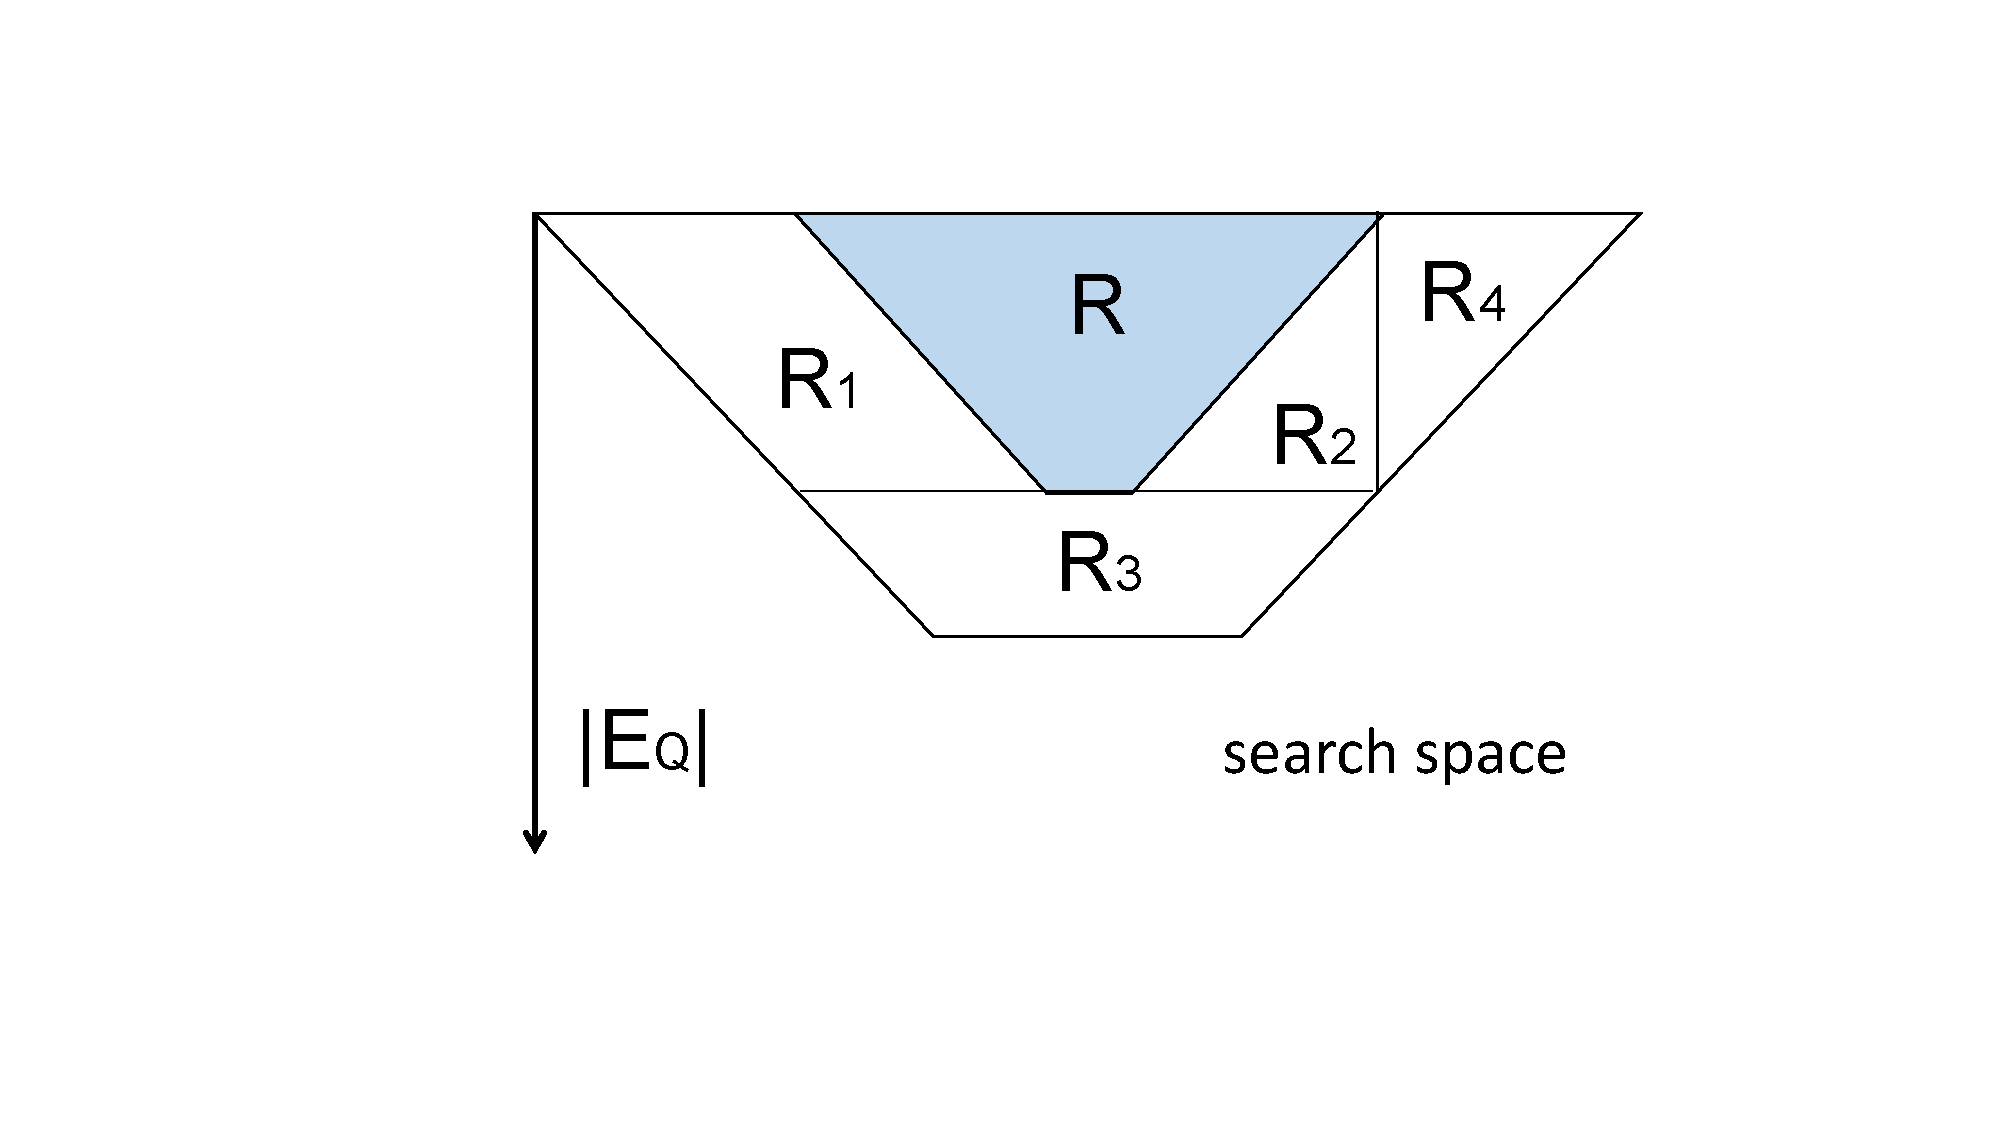
\includegraphics[scale=0.25]{images/search_space}
% \vspace{-2mm}
% \caption{\scriptsize In the whole search space, the smaller trapezoid $R$ is the solution space, and the larger trapezoid, $R+R_1+R_2+R_3+R_4$ is the regions in the search space where $\sigma(Q)\ge$ {\sf Min-sup}.}
% \label{fig:search_space}
% \vspace{-6mm}
% \end{figure}

% \begin{exple}
% 	In Figure \ref{fig:search_space}, to explore the solution region $R$, if expanding by DFS strategy, the region we explore finally will be $R+R_1+R_2+R_3$. If expanding by BFS, the region we explore will be $R+R_1+R_2+R_4$. If we expanding by best-first-search, the region will fit the solution region $R$ as much as possible.
% \end{exple}

% \spara{$\bullet$ DFS lexicographic order edge discovery.} Following the order which is correspond to DFS lexicographic order\cite{YH02} during the new edge discovery, we could guarantee that, the if $Q$ is the first time being discovered, then there must exist $C(Q)=Z(Q)$. Both DFS and BFS strategy of search space expanding could take advantage of this property. What we should guarantee is for any two subgraphs $Q_1,Q_2$, if they have the same edge number, i.e. $|E_{Q_1}|=|E_{Q_2}|$, and $Q_1$ is discovered earlier than $Q_2$, then $Q_1$ must have a smaller DFS lexicographic order. In \cite{YH02}, this property is utilized by carrying out a DFS strategy.
% \begin{figure}[t!]
% \centering
% 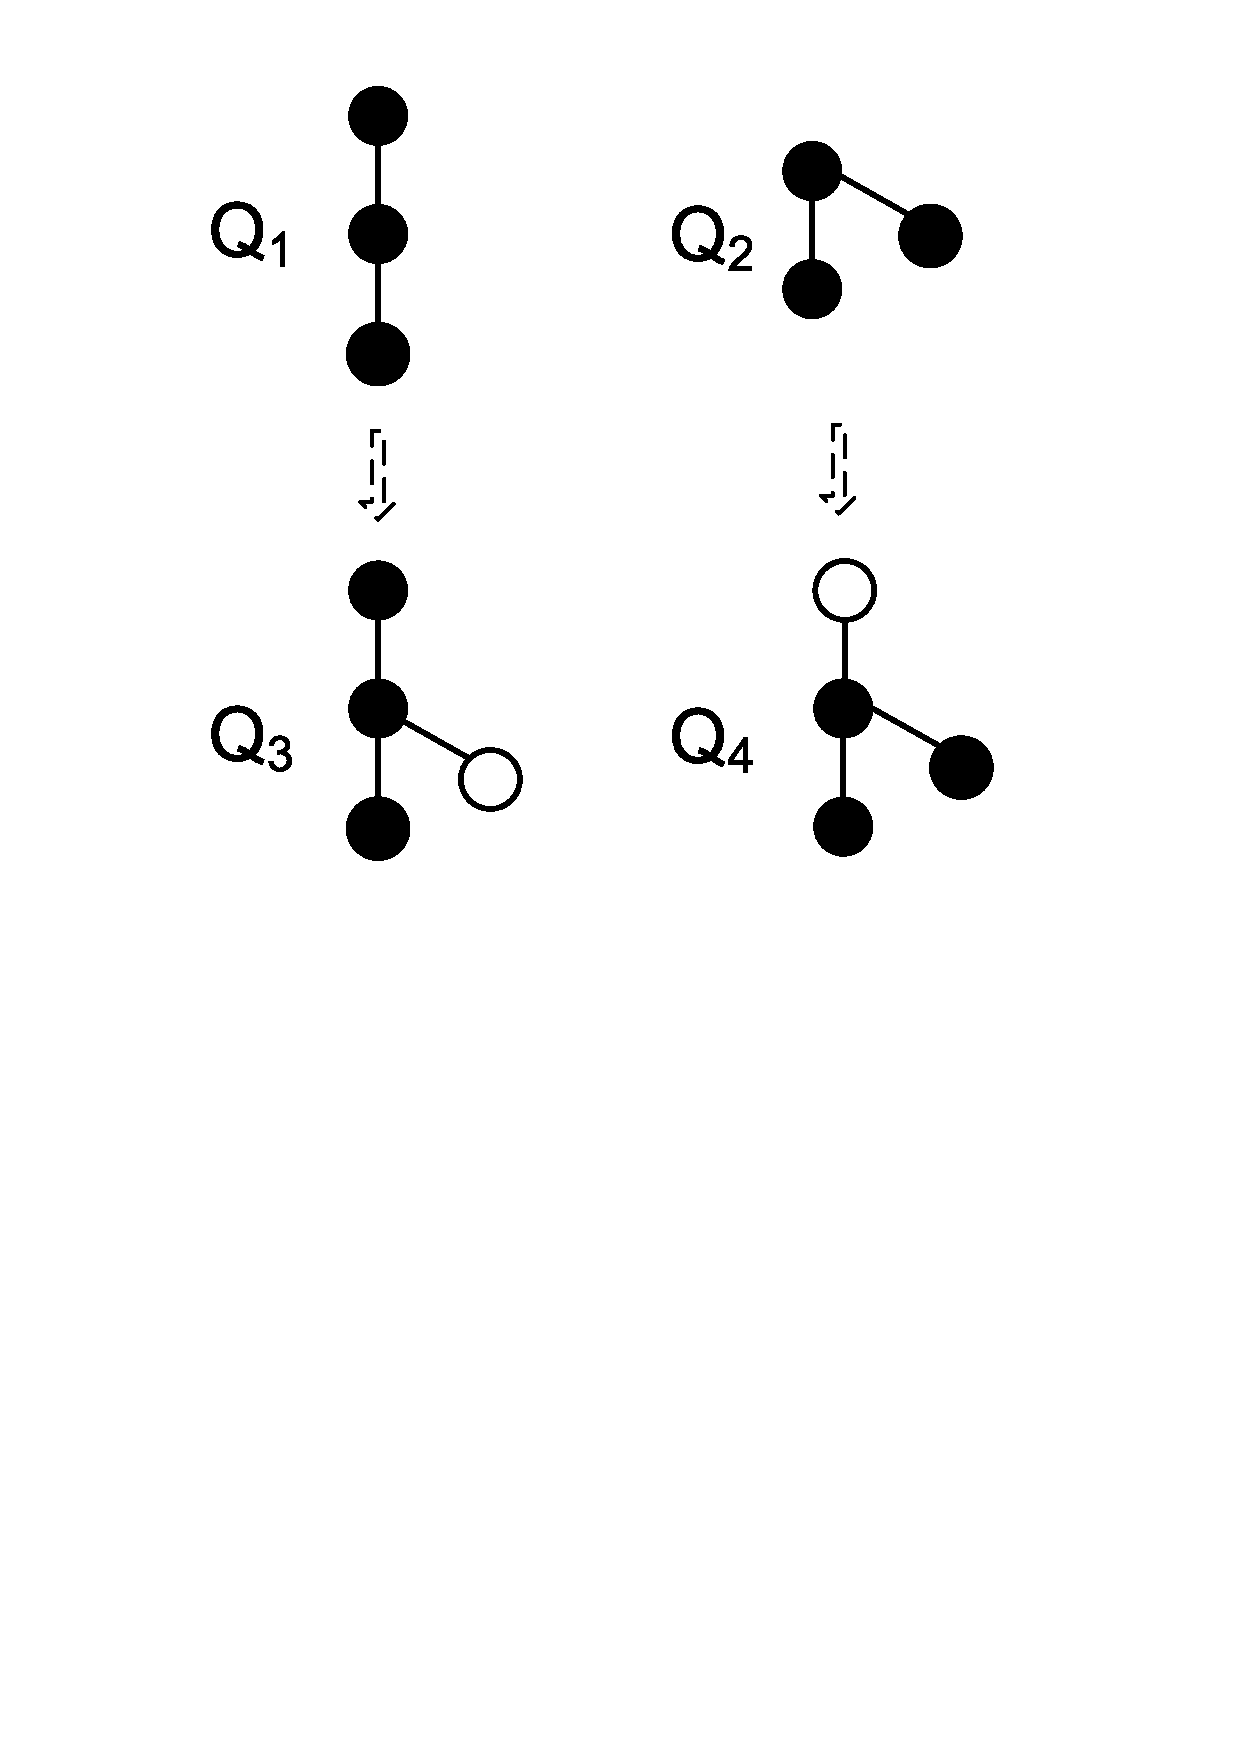
\includegraphics[scale=0.25]{images/lex_order}
% \vspace{-2mm}
% \caption{\scriptsize Subgraph $Q_1$ and $Q_2$ are generated by DFS lexicographic order, i.e. $C(Q_1)=Z(Q_1)$, $C(Q_2)=Z(Q_2)$. $Q_1$ extends to $Q_3$, $Q_2$ extends to $Q_4$, $Q_3,Q_4$ are isomorphic. If follow the DFS lexicographic order, $Q_1$ is discovered earlier than $Q_2$, $Q_3$ is discovered earlier than $Q_4$.}
% \label{fig:lex_order}
% \vspace{-6mm}
% \end{figure}

% \begin{exple}
% 	In Figure \ref{fig:lex_order}, $C(Q_3)=Z(Q_3)$ and $C(Q_4)\not= Z(Q_4)$. To achieve the guarantee above, we should guarantee that $Q_3$ is discovered earlier than $Q_4$. If we expand the search space by DFS, the discovery order is $Q_1,Q_3,Q_2,Q_4$, which satisfies the guarantee. If we expand the search space by BFS, the discovery order is $Q_1,Q_2,Q_3,Q_4$, which satisfies the guarantee. If we expand the search space by best-first-search, since there may exist $\sigma(Q_2)>\sigma(Q_1)$, so that $Q_4$ may be discovered earlier than $Q_3$, which break the guarantee.
% \end{exple}


% Besides, we also consider the disadvantage of best-first-search. If we strictly follow the DFS lexicographic order to generate the subgraph patterns, there is no need to create a dictionary $\mathbb{D}$ because we could prune a subgraph $Q$ directly if $C(Q)\not= Z(Q)$. However, compared with the time cost of generate the minimum DFS code, the search in the dictionary cost only constant time. As a result, the additional time cost of the dictionary is small enough to be ignored. Thus, best-first-search outperform both DFS and BFS without doubt.